\chapter{Introduction}
\label{ch:introduction}

% Why do temperature modeling?
% What level of temperature resolution is needed?
% What temperature resolution is available?
% How can we improve current detectors? (SP)


Since its invention in the 1950's~\citep{carr1954} and later development in the 1970's~\citep{lauterbur1973}, {M}agnetic {R}esonance {I}maging ({MRI}) has allowed physicians and scientists a detailed view within the human body.
  
  % MODELING BOLD
  \section{Models of the fMRI BOLD Response}
  \label{sec:BOLDmodeling}
  
  \begin{figure}[bt]
    \centering
    \vspace{10pt}
    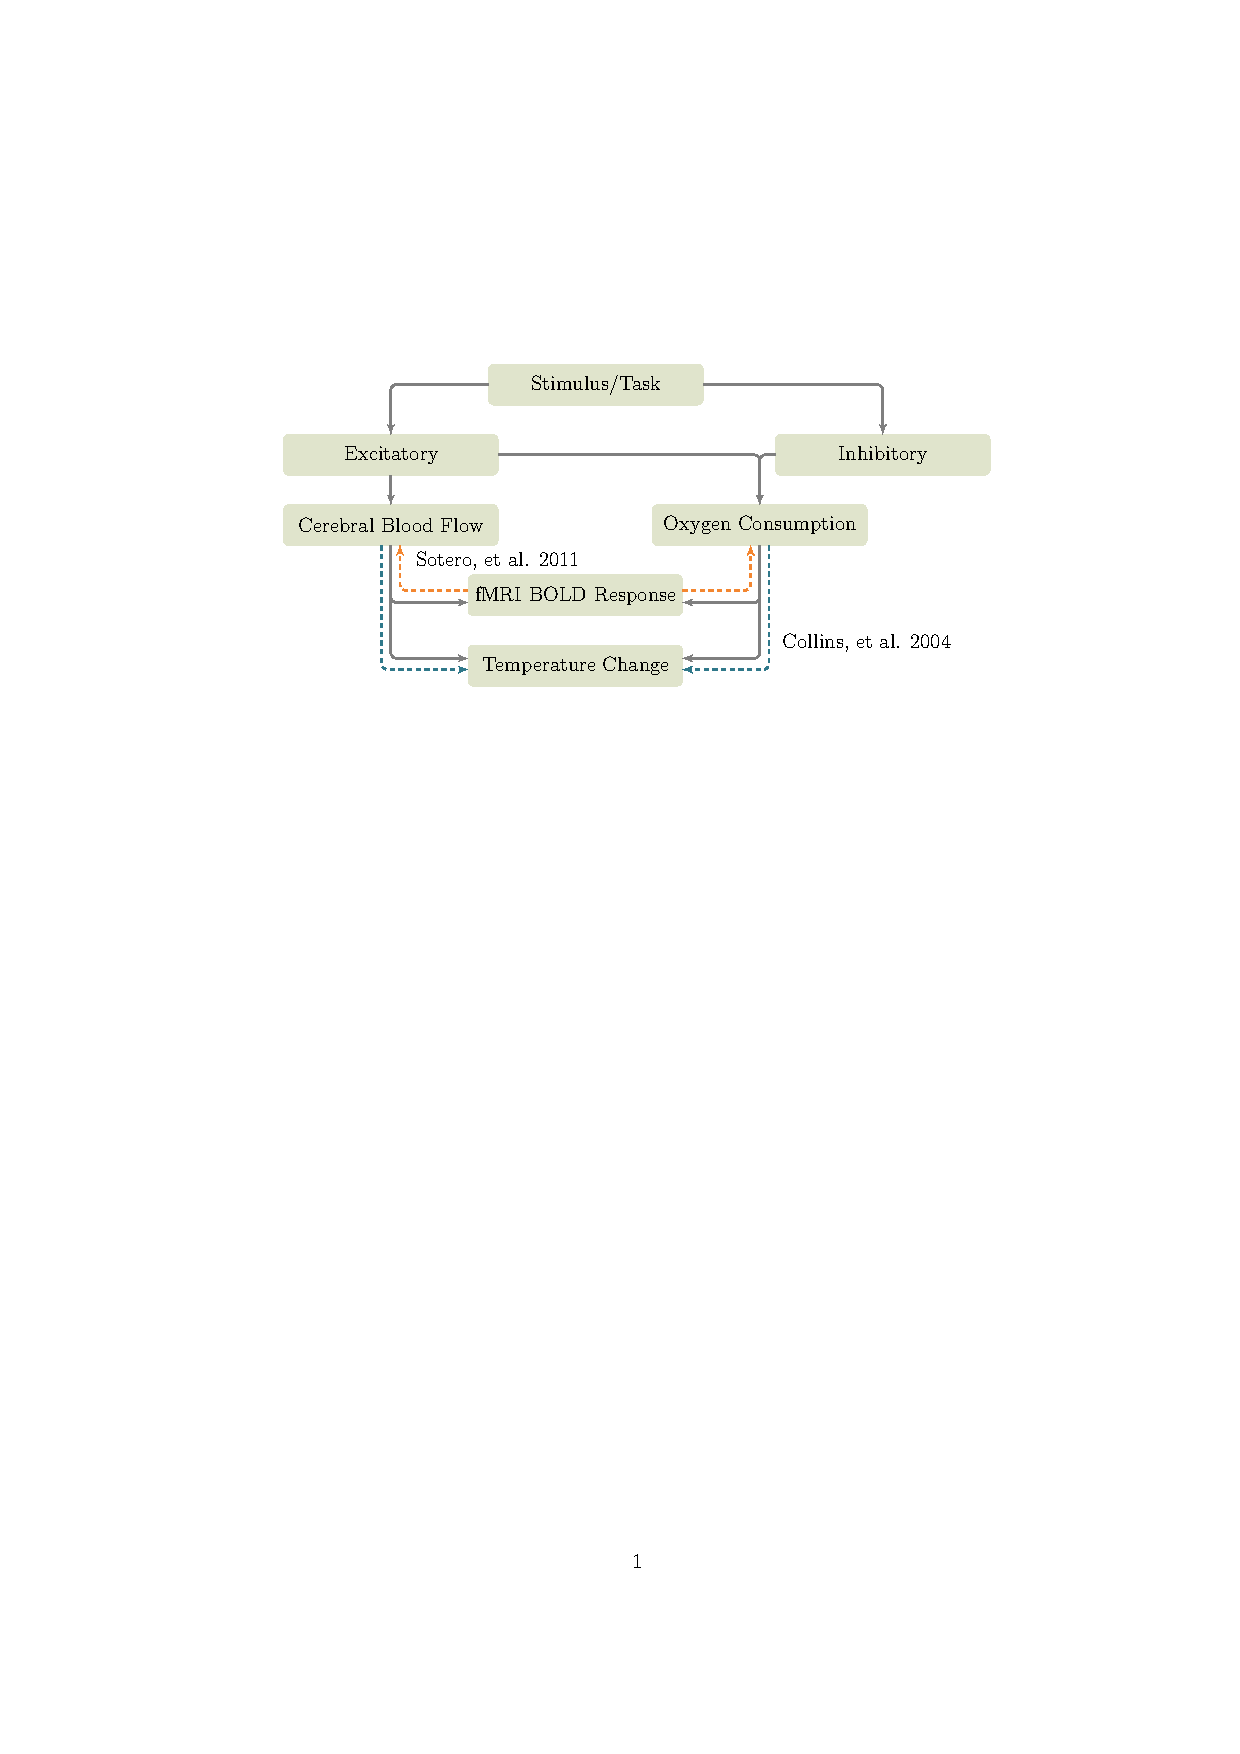
\includegraphics{flowchart}
    % \tikzstyle{block} = [draw=none, fill=beachstorm]
\tikzstyle{line} = [draw, very thick, color=black!50, -stealth']
\tikzstyle{sotero} = [draw, very thick, dashed, color=goldfish, -stealth']
\tikzstyle{collins} = [draw, very thick, dashed, color=aoi, -stealth']
\tikzstyle{citation} = [draw=none, fill=white, minimum height=0.5cm, anchor=north, text width=6.5cm]

\begin{tikzpicture}[node distance=0.7cm, rectangle, text width=4.5cm, text badly centered, rounded corners, minimum height=1cm, anchor=north]
  \node[block](stimulus){Stimulus/Task};
  
  \node[block, below=of stimulus, xshift=-5cm](excitatory){Excitatory Neuronal Activity};
  \node[block, below=of stimulus, xshift= 7cm](inhibitory){Inhibitory Neuronal Activity};
  
  \node[block, below=of excitatory](cbf){Increase in Cerebral Blood Flow (CBF)};
  \node[block, below=of inhibitory, xshift=-3cm](o2){Change in Oxygen Consumption (CMRO$_2$)};
  
  \node[block, below=of cbf, xshift=4.5cm, yshift=-0.5cm](bold){fMRI BOLD Response};
  \node[block, below=of bold](temp){Temperature Change};
  
  \node[citation](sotero1) at (-1.6, -5) {\citet{sotero2011}};
  % \node[citation](sotero1) at (2, -4.5) {Sotero, et. al. 2011};
  % \node[citation](sotero1) at (-4.5, -7.5) {Collins, et. al. 2011};
  \node[citation](sotero1) at (6, -6.5) {\citet{collins}};
  
  \path[line](stimulus.west) -| (excitatory.north);
  \path[line](stimulus.east) -| (inhibitory.north);
  \path[line](excitatory.south) -- (cbf.north);
  \path[line](excitatory.east) -| (o2.north);
  \path[line](inhibitory.west) -| (o2.north);
  
  \path[line](cbf.south) |- ([yshift=-5pt] bold.west);
  \path[line](cbf.south) |- ([yshift= 5pt] temp.west);
  \path[line](o2.south)  |- ([yshift=-5pt] bold.east);
  \path[line](o2.south)  |- ([yshift= 5pt] temp.east);
  
  \path[sotero]([yshift= 5pt] bold) -| ([xshift= 20pt] cbf);
  \path[sotero]([yshift= 5pt] bold) -| ([xshift=-20pt] o2);
  \path[collins]([xshift=-45pt] cbf) |- ([yshift=-5pt] temp);
  \path[collins]([xshift=45pt] o2)  |- ([yshift= -5pt] temp);
\end{tikzpicture}
    \caption[Generation of the fMRI BOLD response and a corresponding temperature change]{\label{fig:flowchart} Generation of the fMRI BOLD response from changes in neuronal activity.  Black arrows indicate a causal relationship while colored dashed-arrows indicate existing models for the relationship.  The orange line ($\color{goldfish}\bullet$) shows the model proposed by~\citet{sotero2011} to calculate cerebral blood flow and metabolism and the blue line ($\color{aoi}\bullet$) shows how the model proposed by~\citet{collins} is used to calculate temperature.}
  \end{figure}
  % Start with Buxton and Friston and build up to how I am calculating the metabolism and blood flow.